\documentclass[12pt,a4paper]{article}
\usepackage{graphicx} % for including images
\usepackage[utf8]{inputenc}
\usepackage{geometry}
\geometry{a4paper, margin=1in}
\usepackage{hyperref} % for hyperlinks

\title{Info2222 Assignment 3 report}
\author{SIDs: 530317166, 510460215}
\date{}

\begin{document}
\maketitle

\section{Introduction}
% Brief introduction to your project and what this document will cover

\section{User Investigation}
\subsubsection*{Persona Overview}
This section presents an analysis of the data collected through a Google Form survey distributed among peers at the University of Sydney. The purpose of the survey was to gather insights to create a detailed persona, which is seen from the table below for our project on enhancing the messaging system used by students.

% Including the persona information as a table
\noindent
\begin{tabular}{|p{0.3\linewidth}|p{0.6\linewidth}|}
\hline
\textbf{Attribute} & \textbf{Details} \\
\hline
\textbf{Photo Name:} & Sam Hong \\
\hline
\textbf{Gender:} & Male \\
\hline
\textbf{Current Role:} & Student \\
\hline
\textbf{Age:} & 20 years \\
\hline
\textbf{Education/Background:} & Second year University of Sydney Computer Science \\
\hline
\textbf{Area of Interest:} & Cybersecurity, AI, and data science \\
\hline
\textbf{Goal and Tasks:} & To efficiently collaborate on group for academic purposes, and being able to message friends and family \\
\hline
\textbf{Environment:} & Owns a desktop and smart phone, has daily uses for messaging applications \\
\hline
\textbf{Quote:} & \textit{"For academic messaging application, I think, as simple desing like a whatsapp is best"} \\
\hline
\end{tabular}


\subsection{Methodology}
The survey was shared using an online Google Form, accessible at \url{https://forms.gle/76AmQiAeyXHEHCMZ7}. It aimed to collect diverse opinions and experiences related to the current messaging systems in use by the students.

\subsection{Demographic and Usage Analysis}
The majority of respondents were male students in their second and third years of study, which provides a clear demographic focus for our user persona. In terms of technology, most respondents reported owning smartphones and desktops, indicating high accessibility to digital platforms. The preferred messaging apps among the participants were Instagram and Discord, which are primarily used for communication between family, friends, and for academic purposes. Furthermore, daily usage of these apps was reported, suggesting a high dependency on digital communication. Regarding navigation preferences, a significant number of users preferred using both mouse and keyboard, which should be considered in designing the interface for enhanced usability.

\subsection{Feedback Analysis}
\subsubsection{Features Lacking in Current Systems}
Participants highlighted several features missing from current messaging systems that could enhance their academic experience:
\begin{itemize}
    \item Customization options such as themes, fonts, and layouts to reduce eye strain.
    \item Better organization features like dedicated channels for different subjects or projects.
    \item Enhanced search functions.
    \item Overall sleeker design.
\end{itemize}

\subsubsection{Challenges Faced}
Respondents identified key challenges with current messaging systems:
\begin{itemize}
    \item Cluttered user interfaces making navigation difficult.
    \item Issues with responsiveness on different devices.
    \item Difficulty tracking important messages in large group chats.
    \item Slow loading times and lack of integration with other academic tools.
\end{itemize}

\subsubsection{Suggested Improvements}
Based on the limitations identified, the following improvements were suggested:
\begin{itemize}
    \item A cleaner, more minimalist design with dropdown menus for complex functions.
    \item Options to tag messages or create threads within chats.
    \item Integration of notifications or reminders for academic deadlines.
    \item Faster loading times and simplified user interface.
\end{itemize}

\section{Navigation Design }
\subsection{Card Sorting}

\begin{itemize}
    \item \textbf{Participants:} The session included 6 participants, comprising of target students
    \item \textbf{Materials:} To simulate cardsorting, participants were provided with a Miro link that contains both sticky notes used as categories and rectangle blocks that were used as cards. 
    \item \textbf{Procedure:} Participants were asked to group these cards into categories that seemed logical to them and then label each category.
\end{itemize}

\subsubsection{Results}
\begin{figure}[h]
\centering
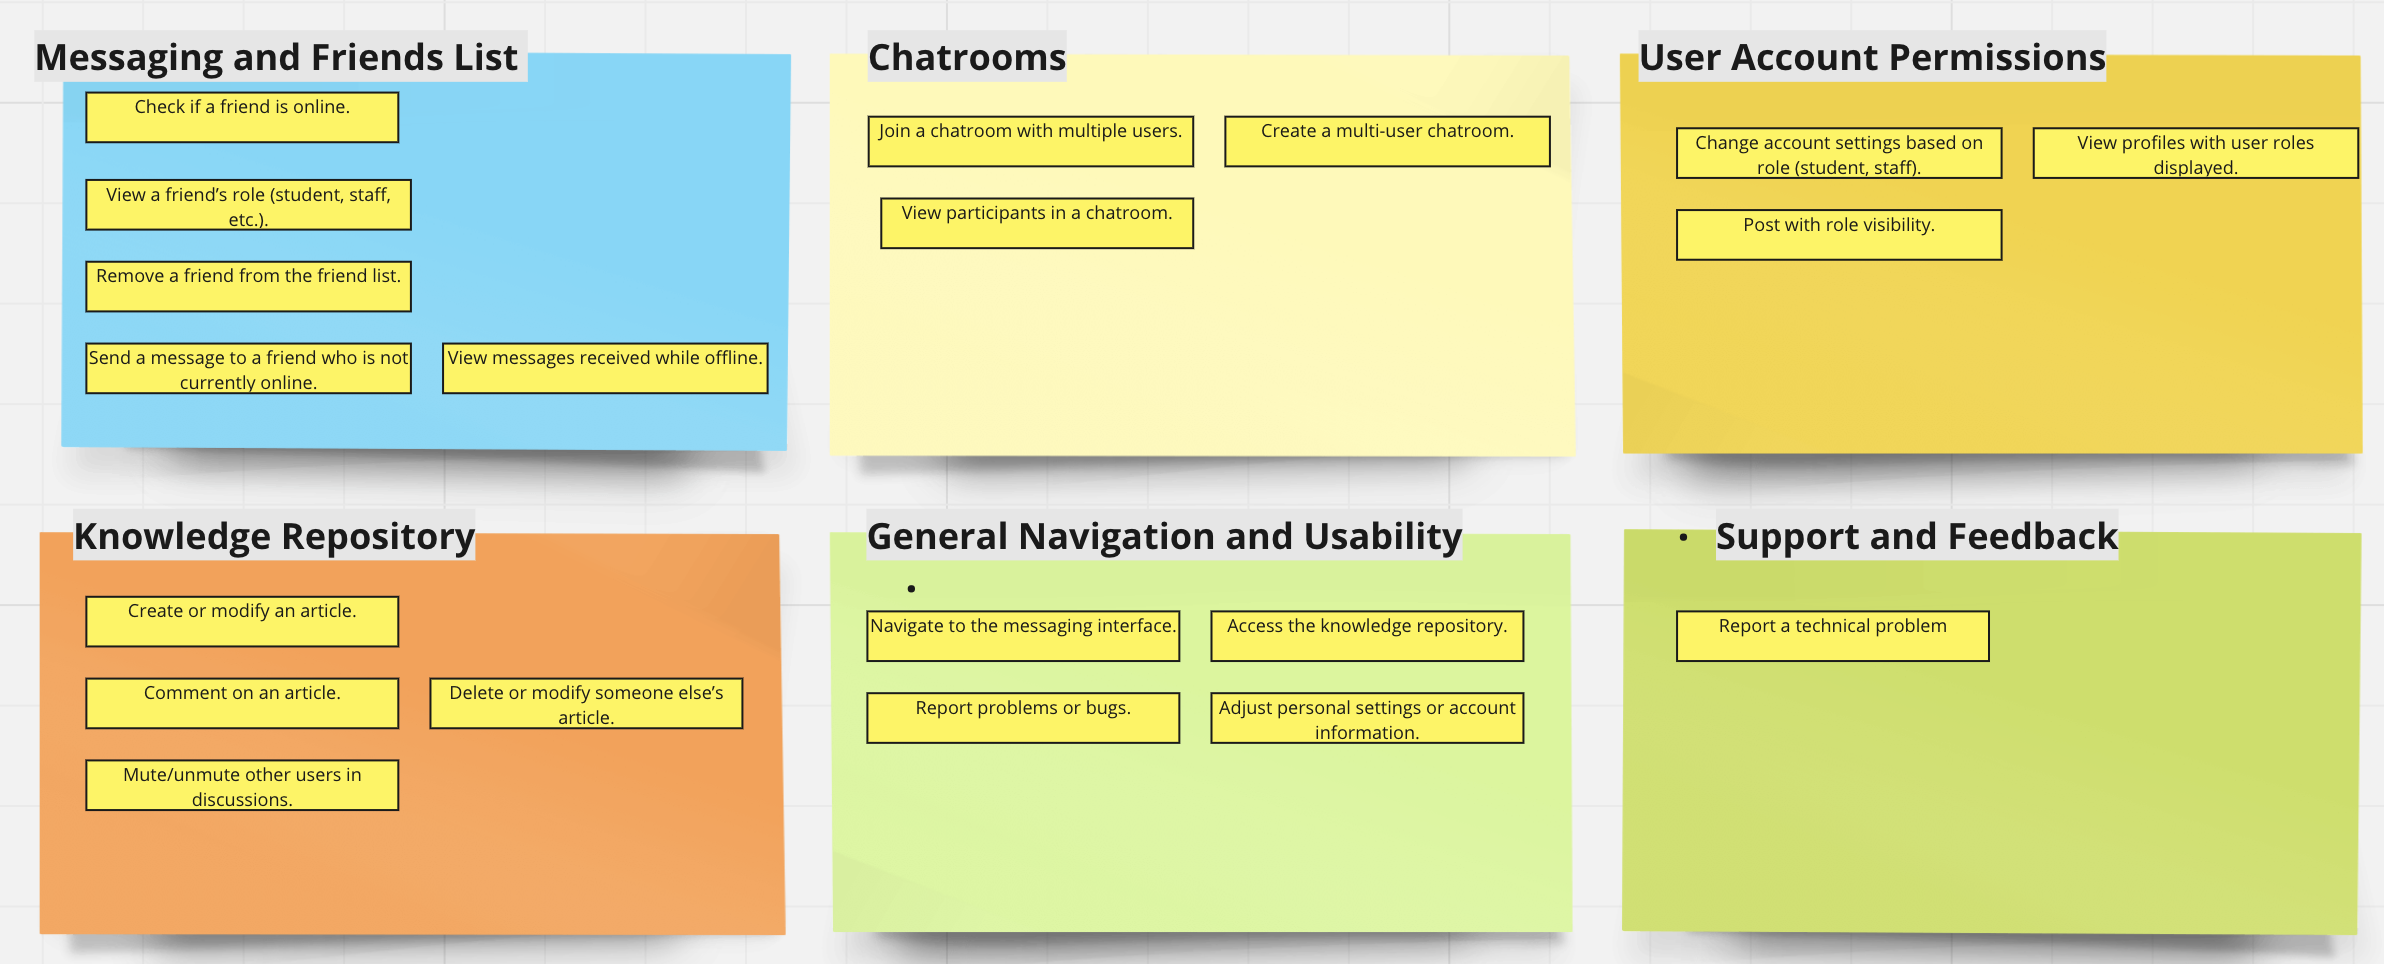
\includegraphics[width=0.8\textwidth]{cardsort.png} 
\caption{Result of cardsort after open and closed card sorting sessions}
\label{fig:sitemap}
\end{figure}


\subsubsection{Information Architecture}
Based on the results of the card sorting session, the following site map was developed to reflect the user-defined categories and expected navigation paths, again, using Miro.

\begin{figure}[h]
\centering
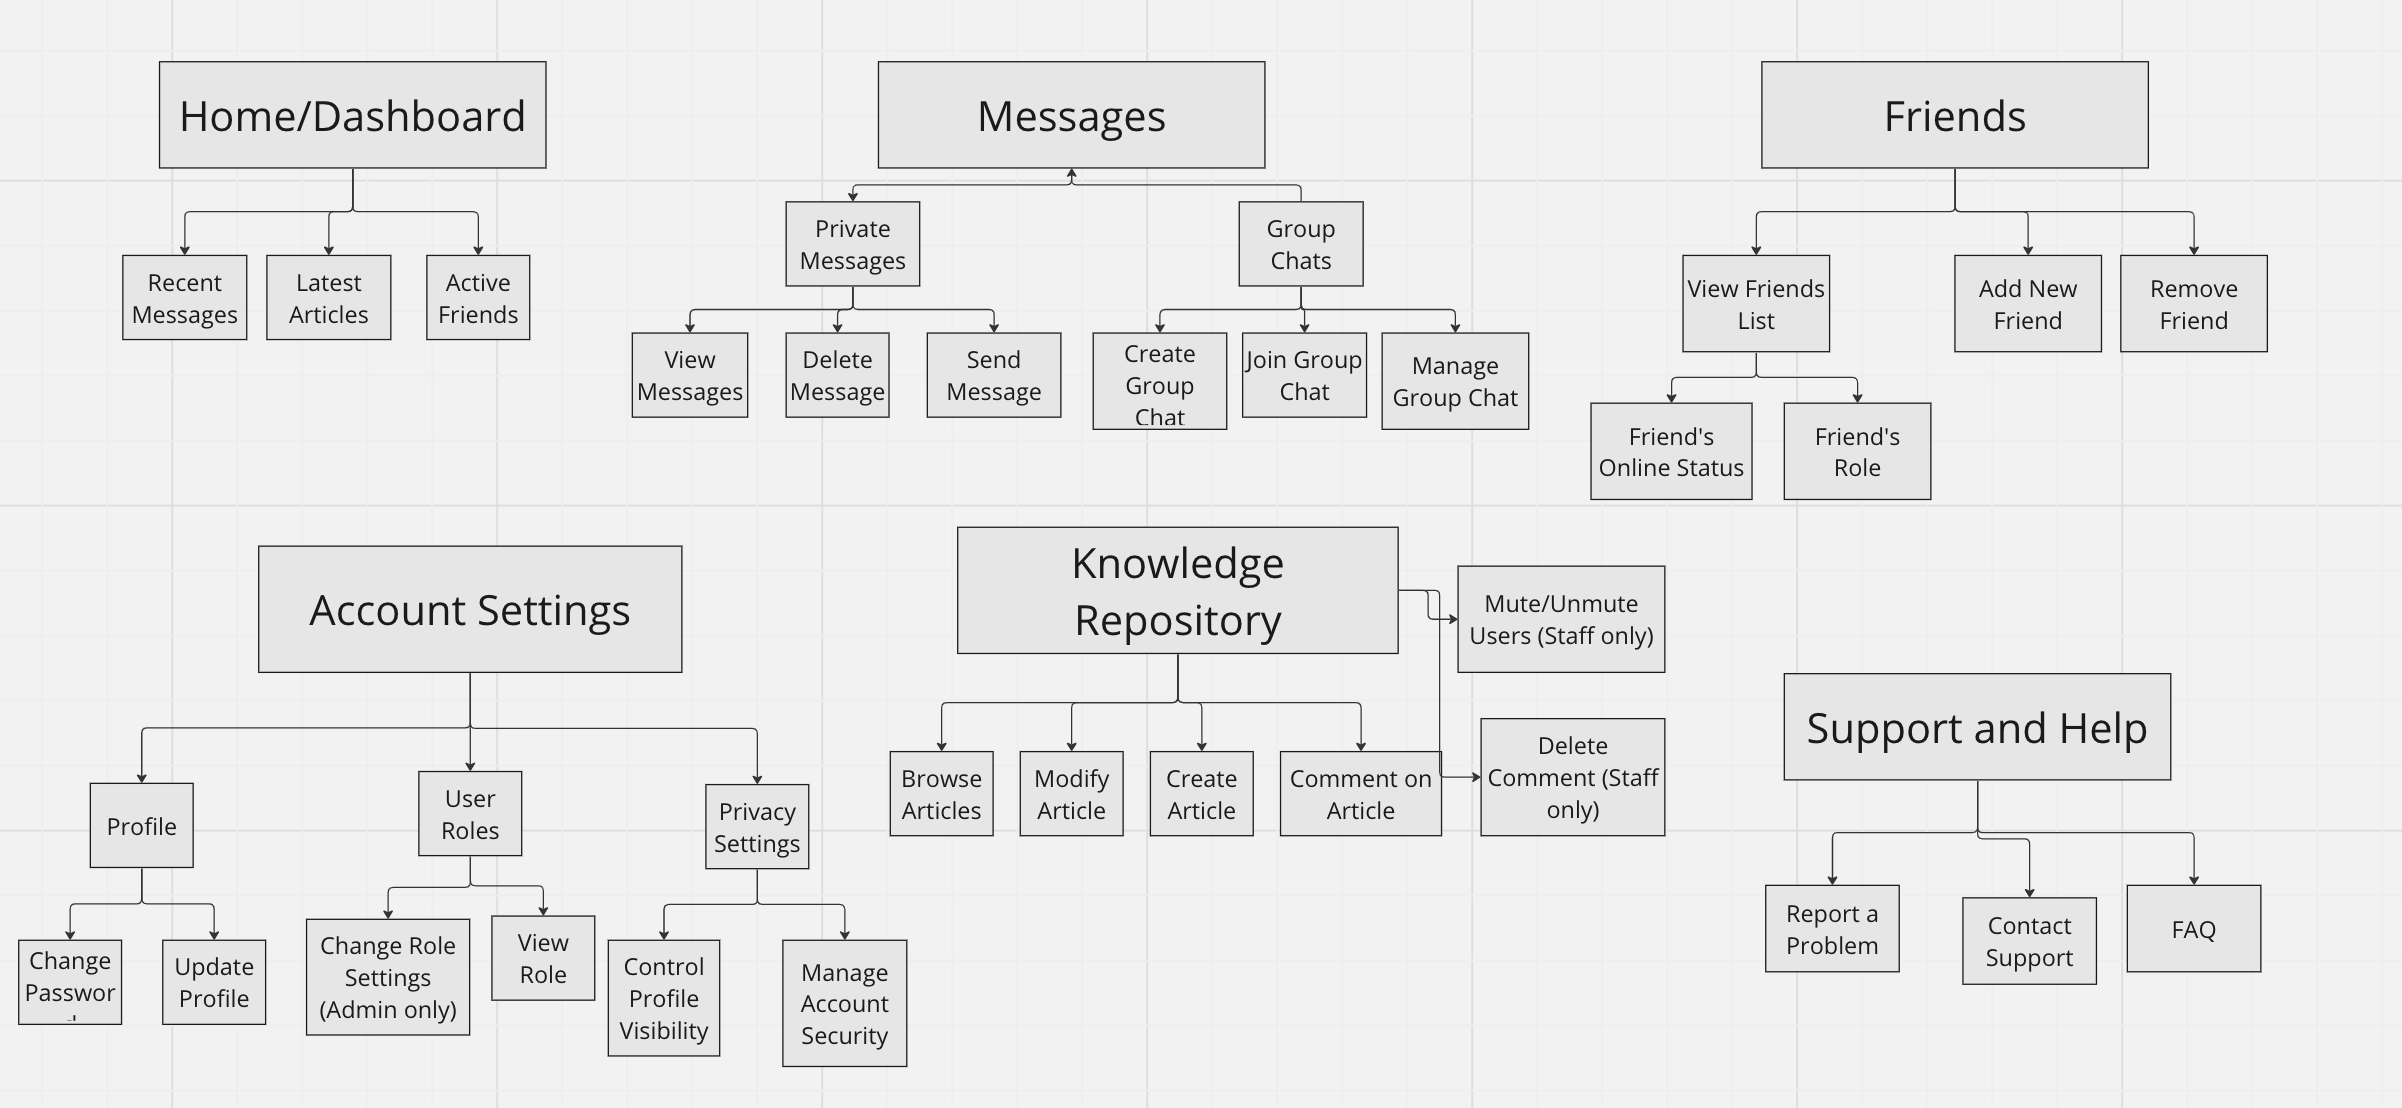
\includegraphics[width=0.8\textwidth]{sitemap.png} % Replace 'sitemap.png' with the actual image file of your site map
\caption{Site Map of the Messaging Platform}
\label{fig:sitemap}
\end{figure}

\section{Design-Evaluate – Low Fidelity or High Fidelity Prototype }
\subsection{Design Process}
Based on the information architecture derived from the card sorting exercise, we brainstormed and developed initial sketches, which were then translated into digital wireframes. The design focused on simplicity and ease of navigation, aligning with user expectations and feedback.

\subsection{Prototype Description}
The prototype was developed using [Prototyping Tool Name], featuring the following key sections:
- \textbf{Home Dashboard}: Quick access to recent messages and updates.
- \textbf{Messages}: Detailed views for private and group chats.
- \textbf{Knowledge Repository}: A section for article browsing and interaction.
- \textbf{Settings}: Account management and privacy settings.

\subsection{Wireframe Diagrams}
\begin{figure}[h]
\centering
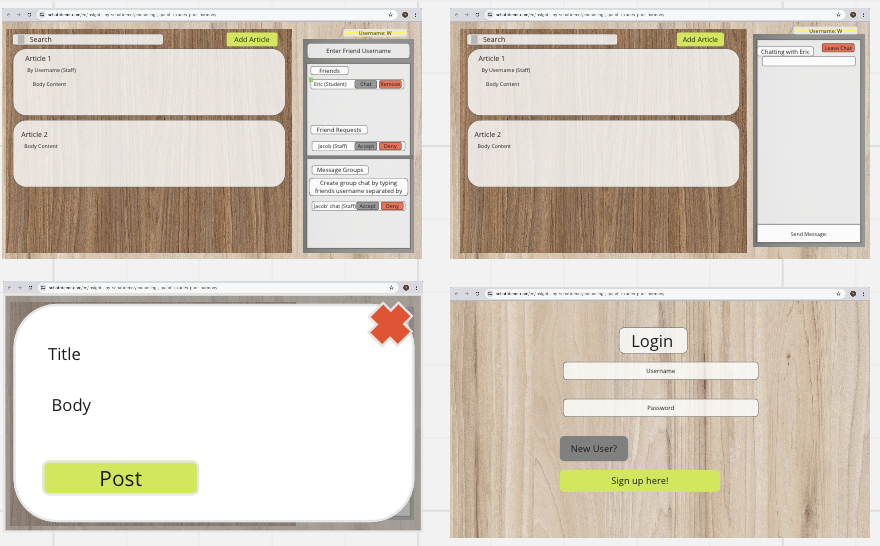
\includegraphics[width=0.8\textwidth]{wireframe.png} % Replace 'wireframe.png' with the actual file name
\caption{Wireframe of the Messaging Platform}
\label{fig:wireframe}
\end{figure}

\subsection{Guerrilla Testing}
\subsubsection{Testing Methodology}
Guerrilla testing was conducted in a common area at the university, where participants were randomly asked to interact with the prototype. Each session lasted approximately 10 minutes, and participants were encouraged to perform specific tasks while voicing their thoughts.

\subsubsection{Participants}
A total of 5 participants were involved, including 4 students from different faculties and 1 administrative staff member, to ensure a diverse range of perspectives.

\subsubsection{Findings and Feedback}
Key feedback from the testing included:
- \textbf{Positive Feedback}: Users appreciated the clear layout and easy navigation.
- \textbf{Suggestions for Improvement}:
  - Increase font size for better readability.
  - Add more intuitive icons for accessing different features.

\subsection{Prioritized Features}
\begin{enumerate}
  \item \textbf{Enhanced Search Functionality}: Critical for quickly finding messages and content within the knowledge repository.
  \item \textbf{Real-Time Notifications}: Important for keeping users informed of new messages and updates.
  \item \textbf{Accessibility Improvements}: Necessary to support users with disabilities, ensuring the platform is usable for everyone.
\end{enumerate}


\end{document}
